% !TeX root = RJwrapper.tex
\title{ppseq: An R Package for Sequential Predictive Probability
Monitoring}
\author{by Emily C. Zabor, Brian P. Hobbs, and Michael J. Kane}

\maketitle

\abstract{%
Clinical trials in oncology are making increasing use of larger phase 1
and phase 2 sample sizes with the addition of baskets for different
disease sub-types or multiple dosing groups, expansion cohorts to
further study safety and obtain preliminary efficacy information, or
randomization to further define efficacy or compare across doses, among
other design elements. With the enlarged sample sizes come increasing
ethical concerns regarding patients who enroll in clinical trials, and
the need for rigorous statistical designs to ensure that trials can stop
early for futility while maintaining traditional control of type I error
and power. The R package \pkg{ppseq} provides a framework for designing
early phase clinical trials using sequential monitoring based on the
Bayesian predictive probability. Trial designs can be compared using
interactive plots and optimized based on efficiency or accuracy.
}

\hypertarget{introduction}{%
\section{Introduction}\label{introduction}}

In the context of cytotoxic treatments, phase 1 trials in oncology
traditionally have the primary aim of identifying the maximum tolerated
dose (MTD), defined as the highest dose that still maintains a certain
pre-specified rate of toxicity, most commonly 30\%, in a dose-escalation
phase. Designs for dose-escalation trials include the rule-based 3+3
design and the model-based continual reassessment method, among others.
But with increasing study focused on non-cytotoxic treatments, such as
immunotherapies, the MTD either may not exist or may not be relevant,
and toxicities may either develop much later or even be chronic, making
these treatments difficult to study with traditional dose-escalation
designs. As a result, it is becoming increasingly common to include
dose-expansion cohorts, in which additional patients are enrolled in
phase 1 after the dose-escalation phase is complete. In this setup, the
dose-escalation phase is considered phase 1a and used to assess the
initial safety of multiple doses, then the dose-expansion phase is
considered phase 1b and can have a variety of aims including to further
refine the safety of one or more doses, to assess preliminary efficacy,
to explore the treatment in various disease-specific subtypes that all
share a common biomarker that the treatment is targeting, or to further
characterize the pharmacokinetics and/or pharmacodynamics. The use of
dose-expansion cohorts increased from 12\% in 2006 to 38\% in 2011
\citep{Manji2013} and trials with dose-expansion cohorts led to higher
response rates and more frequent success in phase 2 trials
\citep{Bugano2017}.

But dose-expansion cohorts are not always planned in advance, and
therefore may be subject to on-the-fly decision making that can lead to
large sample sizes and poor statistical properties. For example, the
KEYNOTE-001 trial of pembrolizumab, initially designed as a 3+3
dose-escalation trial, included multiple protocol amendments and
ultimately enrolled a total of 495 non-small-cell lung cancer patients
across six disease-specific expansion cohorts \citep{Garon2015}. In a
basket trial of atezolizumab, an anti-PD-L1 treatment in patients with a
variety of cancers and both with and without PD-L1 expression, an
expansion cohort in metastatic urothelial bladder cancer ultimately
enrolled 95 patients, despite the fact that no expansion cohort in this
disease subtype was originally planned in the trial protocol but was
rather added later in a protocol amendment in which the sample size was
increased from what was initially planned
\citep{Petrylak2018, Powles2014}.

Bayesian sequential predictive probability monitoring provides a natural
framework for early phase oncology trial design, allowing flexibility to
stop early for futility or safety concerns while also maintaining
traditional levels of power and control of type I error, and has been
proposed as an approach to interim monitoring in clinical trials
previously {[}\citet{Dmitrienko2006}; Lee2008; Saville2014{]}. However,
in order to be useful to investigators designing such trials, software
must be made available that streamlines design. This paper introduces
the \pkg{ppseq} package for the R software language \citep{RCT2020},
which provides functions to design one-sample and two-sample early phase
clinical trials using sequential predictive probability monitoring.
Interactive plots produced using \CRANpkg{ggplot2} and \CRANpkg{plotly}
assist investigators in comparing designs based on different thresholds
for decision making, and we suggest optimization criteria for selecting
the ideal design.

\hypertarget{predictive-probability-monitoring}{%
\section{Predictive probability
monitoring}\label{predictive-probability-monitoring}}

Consider the setting of a binary outcome, such as tumor response as
measured by the RECIST criteria in the setting of a study in patients
with solid tumors, where each patient, denoted by \(i\), enrolled in the
trial either has a response such that \(x_i = 1\) or does not have a
response such that \(x_i = 0\). Then \(X = \sum_{i=1}^n x_i\) represents
the number of responses out of \(n\) currently observed patients up to a
maximum of \(N\) total enrolled patients. Let \(p\) represent the
probability of response, where \(p_0\) represents the null response rate
under no treatment or the standard of care treatment and \(p_1\)
represents the alternative response rate under the experimental
treatment. Most dose-expansion studies with an efficacy aim will wish to
test the null hypothesis \(H_0: p \leq p_0\) versus the alternative
hypothesis \(H_1: p \geq p_1\).

The Bayesian paradigm of statistics is founded on Bayes rule, which is a
mathematical theory that specifies how to combine the prior
distributions that define prior beliefs about parameters, such as the
response rate \(p\), with the observed data, such as the total number of
responses \(X\), yielding a posterior distribution. Here the prior
distribution of the response rate \(\pi(p)\) has a beta distribution
\(Beta(a_0, b_0)\) and our data \(X\) have a binomial distribution
\(bin(n, p)\). Combining the likelihood function for the observed data
\(L_x(p) \propto p^x (1-p)^{n-x}\) with the prior, we obtain the
posterior distribution of the response rate, which follows the beta
distribution \(p|x \sim Beta(a_0 + x, b_0 + n - x)\). Using the
posterior probability, which represents the probability of success based
only on the data accrued so far, we would declare a treatment
efficacious if \(\Pr(p>p_0 | X) > \theta\), where \(\theta\) represents
a pre-specified posterior decision threshold. The posterior predictive
distribution of the number of future responses \(X^*\) in the remaining
\(n^*=N-n\) future patients follows a beta-binomial distribution
\(Beta-binomial(n^*, a_0 + x, b_0 + n - x)\). Then the posterior
predictive probability (PPP), is calculated as
\(PPP = \sum_{{x^*}=0}^{n^*} \Pr(X^*=x^*|x) \times I(\Pr(p>p_0 | X, X^*=x^*) > \theta)\).
The posterior predictive probability represents the probability that the
treatment will be declared efficacious at the end of the trial when full
enrollment is reached. We would stop the trial early for futility if the
posterior predictive probability dropped below a pre-specified threshold
\(\theta^*\), i.e.~\(PPP<\theta^*\). Predictive probability thresholds
closer to 0 lead to less frequent stopping for futility whereas
thresholds near 1 lead to frequent stopping unless there is almost
certain probability of success. Predictive probability provides an
intuitive interim monitoring strategy for clinical trials that tells the
investigator what the chances are of declaring the treatment efficacious
at the end of the trial if we were to continue enrolling to the maximum
planned sample size, based on the data observed in the trial to date.

\hypertarget{package-overview}{%
\section{Package overview}\label{package-overview}}

The \pkg{ppseq} package facilitates the design of clinical trials
utilizing sequential predictive probability monitoring. The main
challenge in designing such a trial is joint calibration of the
posterior probability and posterior predictive probability thresholds to
be used in the trial in order to maintain the desired level of power and
type I error. The \code{calibrate\_thresholds()} function will evaluate
a grid of posterior and predictive thresholds provided by the user as
vector inputs through the argument \code{pp\_threshold} for posterior
thresholds and the argument \code{ppp\_threshold} for predictive
thresholds. Other required arguments include the null response rate
\code{p\_null}, the alternative response rate \code{p\_alt}, a vector of
sample sizes at which interim analyses are to be performed \code{n} as
well as the maximum total sample size \code{N}, the direction of the
alternative hypothesis \code{direction}, a vector of the two
hyperparameters of the prior beta distribution \code{prior}, and the
number of posterior samples \code{S} and the number of simulated trial
datasets \code{nsim}. The additional argument \code{delta} can specify
the clinically meaningful difference between groups in the case of a
two-sample trial design. The function returns a list, the first element
of which is a \code{tibble} containing the posterior threshold,
predictive threshold, the mean sample size under the null and the
alternative, the proportion of positive trials under the null and
alternative, and the proportion of trials stopped early under the null
and alternative. The proportion of positive trials under the null
represents the type I error and the proportion of positive trials under
the alternative represents the power. The \code{print()} option will
print the results summary for each combination of thresholds, filtered
by an acceptable range of type I error and minimum power, if desired.

\hypertarget{optimization}{%
\subsection{Optimization}\label{optimization}}

After obtaining results for the all combinations of evaluated posterior
and predictive thresholds, the next step is to select the ideal design
from among the various options. The \pkg{ppseq} package introduces two
optimization criteria to assist users in making a selection. The first,
called the ``optimal accuracy'' design, identifies the design that
minimizes the Euclidean distance to the top left point on a plot of the
type I error by the power. The second, called the ``optimal efficiency''
design, identifies the design that minimizes the Euclidean distance to
the top left point on a plot of the average sample size under the null
by the average sample size under the alternative, subject to constraints
on the type I error and power. The \code{optimize\_design()} function
will return a list that contains the details of each of the two optimal
designs.

\hypertarget{decision-rules}{%
\subsection{Decision rules}\label{decision-rules}}

To ease the implementation of clinical trials designed with sequential
predictive probability monitoring, once a design has been selected, a
table of decision rules can be produced using the
\code{calc\_decision\_rules()} function. The function takes the sample
sizes \code{n} at which interim analyses are to be performed as well as
the maximum total sample size \code{N}, the null value to compare to in
the one-sample case \code{p0} (set to \code{NULL} in the two-sample
case), the posterior threshold of the selected design \code{theta}, the
predictive threshold of the selected design \code{ppp}, the direction of
the alternative hypothesis \code{direction}, a vector of the two
hyperparameters of the prior beta distribution \code{prior}, and the
number of posterior samples \code{S}. The additional argument
\code{delta} can specify the clinically meaningful difference between
groups in the case of a two-sample trial design (set to \code{NULL} in
the one-sample case). The function results in a \code{tibble}. In the
one-sample case, the \code{tibble} includes a column for the sample size
\code{n} at each interim analysis, a column for the decision point
\(r\), and a column for the posterior predictive probability associated
with that decision \code{ppp}. The trial would stop at a given look if
the number of observed responses is \(\leq r\) otherwise the trial would
continue enrolling if the number of observed responses is \(>r\). At the
end of the trial when the maximum planned sample size is reached, the
treatment would be considered promising if the number of observed
responses is \(>r\). In the two-sample case, the \code{tibble} includes
columns for \code{n0} and \code{n1}, the sample size at each interim
analysis in the control and experimental arms, respectively, columns for
\code{r0} and \code{r1}, the number of responses in the control arm and
experimental arm leading to the decision, respectively,and a column for
the posterior predictive probability associated with that decision
\code{ppp}.

\hypertarget{visualizations}{%
\subsection{Visualizations}\label{visualizations}}

Finally, to assist users in comparing the results of the various design
options, a \code{plot()} option is available for the results of
\code{calibrate\_thresholds} that allows creation of static plots using
the \CRANpkg{ggplot2} package \citep{Wickham2016} or interactive plots
using the \CRANpkg{plotly} package \citep{Sievert2020}. Two plots are
produced, one plotting type I error by power and indicating the optimal
accuracy design, and one plotting the average sample size under the null
by the average sample size under the alternative and indicating the
optimal efficiency design. The motivation for including an interactive
graphics option was the utility of the additional information available
when hovering over each point. Instead of simply eyeballing where points
fall along the axes, users can see the specific type I error, power,
average sample size under the null, average sample size under the
alternative, the posterior and predictive thresholds associated with the
design, as well as the distance to the upper left point on the plot. A
\code{plot()} option is also available for the results of
\code{calc\_decision\_rules}. In the one-sample case it produces a
single plot showing the sample size at each interim analysis on the
x-axis and the possible number of responses at each interim analysis on
the y-axis. In the two-sample case a grid of plots is produced, with one
plot for each interim analysis. The x-axis shows the number of possible
responses in the control group and the y-axis shows the number of
possible responses in the experimental group. In both cases, the boxes
are colored green for a ``proceed'' decision and red for a ``stop''
decision for each combination and the hover box produced by
\CRANpkg{plotly} provides the details.

\hypertarget{case-study}{%
\section{Case study}\label{case-study}}

To demonstrate the functionality of the \pkg{ppseq} package, we focus on
a re-design of a dose-expansion cohort for the study of atezolizumab in
metastatic urothelial carcinoma patients (mUC) using sequential
predictive probability monitoring. Atezolizumab is an anti-PD-L1
treatment that was originally tested in the phase 1 setting in a basket
trial across a variety of cancer sites harboring PD-L1 mutations. The
atezolizumab expansion study in mUC had the primary aim of further
evaluating safety, pharmacodynamics and pharmacokinetics and therefore
was not designed to meet any specific criteria for type I error or
power. An expansion cohort in mUC was not part of the original protocol
design, but was rather added later through a protocol amendment. The
expansion cohort in mUC ultimately enrolled a total of 95 participants
\citep{Powles2014}. Other expansion cohorts that were included in the
original protocol, including in renal-cell carcinoma, non-small-cell
lung cancer, and melanoma, were planned to have a sample size of 40.
These pre-planned expansion cohorts were designed with a single interim
analysis for futility that would stop the trial if 0 responses were seen
in the first 14 patients enrolled. According to the trial protocol, this
futility rule is associated with at most a 4.4\% chance of observing no
responses in 14 patients if the true response rate is 20\% or higher.
The protocol also states the widths of the 90\% confidence intervals for
a sample size of 40 if the observed response rate is 30\%. There was no
stated decision rule for efficacy since efficacy was not an explicit aim
of the expansion cohorts. In the re-design we assume a null, or
unacceptable, response rate of 0.1 and an alternative, or acceptable,
response rate of 0.2. We plan a study with up to a total of 95
participants. In our sequential predictive probability design we will
check for futility after every 5 patients are enrolled. We consider
posterior thresholds of 0, 0.7, 0.74, 0.78, 0.82, 0.86, 0.9, 0.92, 0.93,
0.94, 0.95, 0.96, 0.97, 0.98, 0.99, 0.999, 0.9999, 0.99999, and 1, and
predictive thresholds of 0.05, 0.1, 0.15, and 0.2.

First we install and load the \pkg{ppseq} package.

\begin{Schunk}
\begin{Sinput}
install.packages("ppseq")
\end{Sinput}
\end{Schunk}

\begin{Schunk}
\begin{Sinput}
library(ppseq)
\end{Sinput}
\end{Schunk}

We use the \code{calibrate\_thresholds()} function to obtain the
operating characteristics of designs based on on each combination of
posterior and predictive thresholds. Because of the inherent computation
intensity in these calculations, this function relies on the
\CRANpkg{future} \citep{Bengtsson2020} and \CRANpkg{furrr}
\citep{Vaughan2021} packages to parallelize computations. The user will
be responsible for setting up a call to \code{future::plan()} that is
appropriate to their operating environment and simulation setting. The
example in this case study was run on a Unix server with 192 cores, and
we wished to use 76 cores to accommodate the 76 distinct designs that
result from the 19 posterior by 4 predictive threshold grid. Because the
code takes some time to run, the results of the below example code are
available as a dataset called \code{one\_sample\_cal\_tbl} included in
the \pkg{ppseq} package.

\begin{Schunk}
\begin{Sinput}
library(future)

set.seed(123)

plan(multicore(workers = 76))

one_sample_cal_tbl <- 
  calibrate_thresholds(
    p_null = 0.1, 
    p_alt = 0.2, 
    n = seq(5, 95, 5),
    N = 95, 
    pp_threshold = c(0, 0.7, 0.74, 0.78, 0.82, 0.86, 0.9, 0.92, 0.93, 0.94, 
                     0.95, 0.96, 0.97, 0.98, 0.99, 0.999, 0.9999, 0.99999, 1),
    ppp_threshold = seq(0.05, 0.2, 0.05),
    direction = "greater", 
    delta = NULL, 
    prior = c(0.5, 0.5), 
    S = 5000, 
    nsim = 1000
    )
\end{Sinput}
\end{Schunk}

Next we print the results table using the \code{print()} option, and
limited to designs with type I error between 0.01 and 0.2, and a minimum
power of 0.7. We find that 35 of the 76 designs meet these criteria for
type I error and power.

\begin{Schunk}
\begin{Sinput}
print(
  one_sample_cal_tbl,
  type1_range = c(0.01, 0.2),
  minimum_power = 0.7
  )
\end{Sinput}
\begin{Soutput}
#> # A tibble: 35 x 8
#>    pp_threshold ppp_threshold mean_n1_null prop_pos_null prop_stopped_null
#>           <dbl>         <dbl>        <dbl>         <dbl>             <dbl>
#>  1         0.7           0.1          18.2         0.199             0.543
#>  2         0.7           0.15         16.7         0.182             0.728
#>  3         0.7           0.2          11.6         0.139             0.801
#>  4         0.74          0.1          18.1         0.199             0.544
#>  5         0.74          0.15         16.7         0.182             0.728
#>  6         0.74          0.2          11.6         0.139             0.801
#>  7         0.78          0.1          18.1         0.200             0.544
#>  8         0.78          0.15         16.7         0.182             0.728
#>  9         0.78          0.2          11.6         0.139             0.801
#> 10         0.82          0.1          18.1         0.200             0.544
#> # ... with 25 more rows, and 3 more variables: mean_n1_alt <dbl>,
#> #   prop_pos_alt <dbl>, prop_stopped_alt <dbl>
\end{Soutput}
\end{Schunk}

We use the \code{optimize\_designs()} function to obtain the details of
the optimal accuracy and optimal efficiency designs, limited to our
desired range of type I error and minimum power. We find that the
optimal accuracy design is the one with posterior threshold 0.9 and
predictive threshold 0.05. It has a type I error of 0.072, power of
0.883, average sample size under the null of 51, and average sample size
under the alternative of 91. The optimal efficiency design is the one
with posterior threshold of 0.92 and predictive threshold of 0.1. It has
a type I error of 0.06, power of 0.796, average sample size under the
null of 39, and average sample size under the alternative of 82. For
comparison, the original design of the atezolizumab expansion cohort in
mUC, with a single look for futility after the first 14 patients, has a
type I error of 0.005, power of 0.528, average sample size under the
null of 76, and average sample size under the alternative of 92.

\begin{Schunk}
\begin{Sinput}
optimize_design(
  one_sample_cal_tbl, 
  type1_range = c(0.05, 0.1), 
  minimum_power = 0.7
  )
\end{Sinput}
\begin{Soutput}
#> $`Optimal accuracy design:`
#> # A tibble: 1 x 6
#>   pp_threshold ppp_threshold `Type I error` Power `Average N under the null`
#>          <dbl>         <dbl>          <dbl> <dbl>                      <dbl>
#> 1         0.93           0.1         0.0872 0.890                       16.7
#>   `Average N under the alternative`
#>                               <dbl>
#> 1                              24.3
#> 
#> $`Optimal efficiency design:`
#> # A tibble: 1 x 6
#>   pp_threshold ppp_threshold `Type I error` Power `Average N under the null`
#>          <dbl>         <dbl>          <dbl> <dbl>                      <dbl>
#> 1         0.93          0.15         0.0692 0.780                       11.6
#>   `Average N under the alternative`
#>                               <dbl>
#> 1                              21.5
\end{Soutput}
\end{Schunk}

To compare these optimal designs with all other designs, we can use the
\code{plot()} function with the \code{plotly = TRUE} option to obtain
interactive visualizations.

\begin{Schunk}
\begin{Sinput}
plot(
  one_sample_cal_tbl, 
  type1_range = c(0.01, 0.2), 
  minimum_power = 0.7,
  plotly = TRUE
  )
\end{Sinput}
\end{Schunk}

\begin{Schunk}

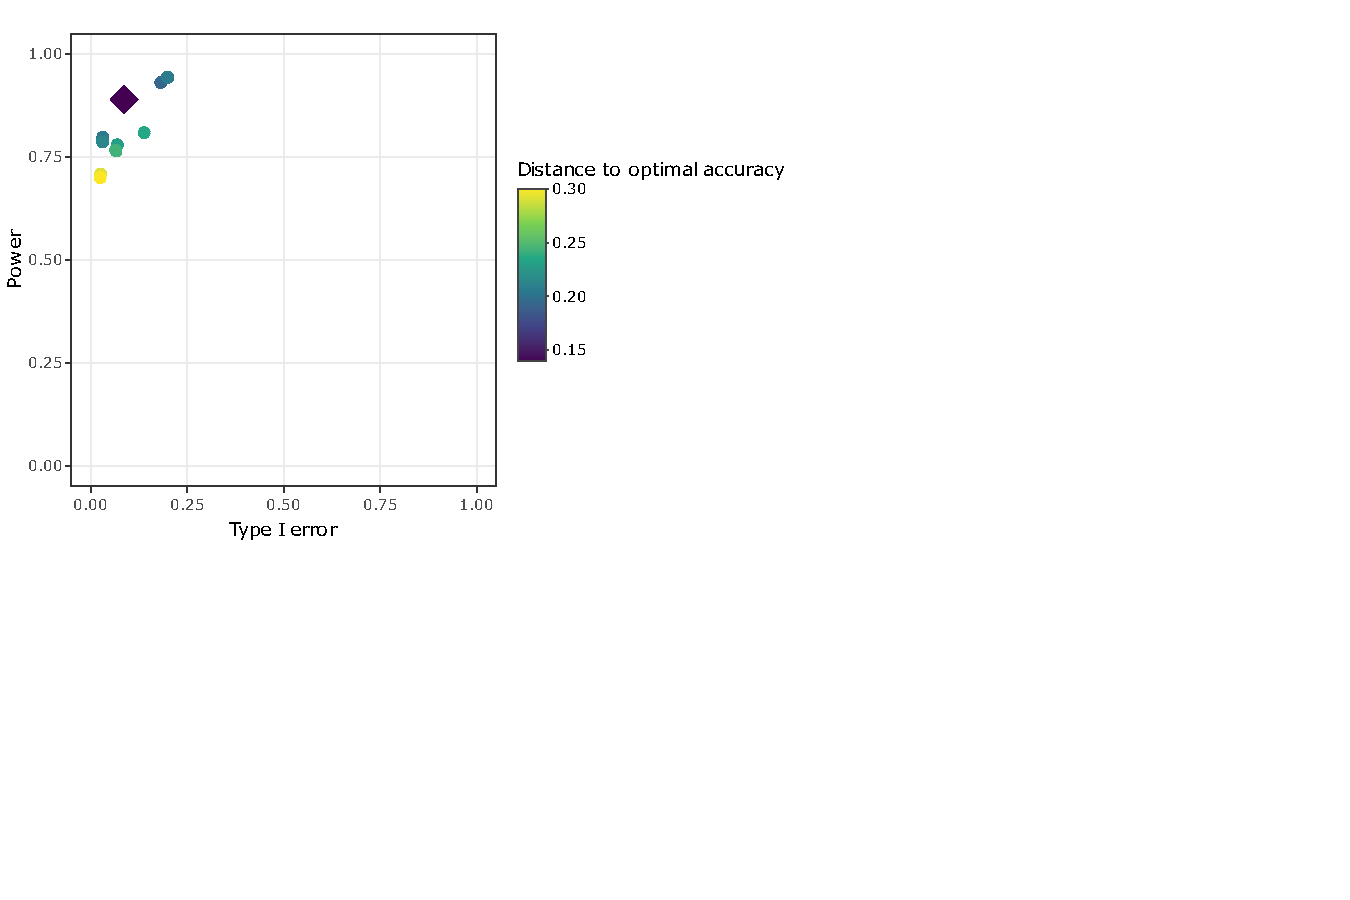
\includegraphics{zabor-hobbs-kane_files/figure-latex/unnamed-chunk-7-1} 
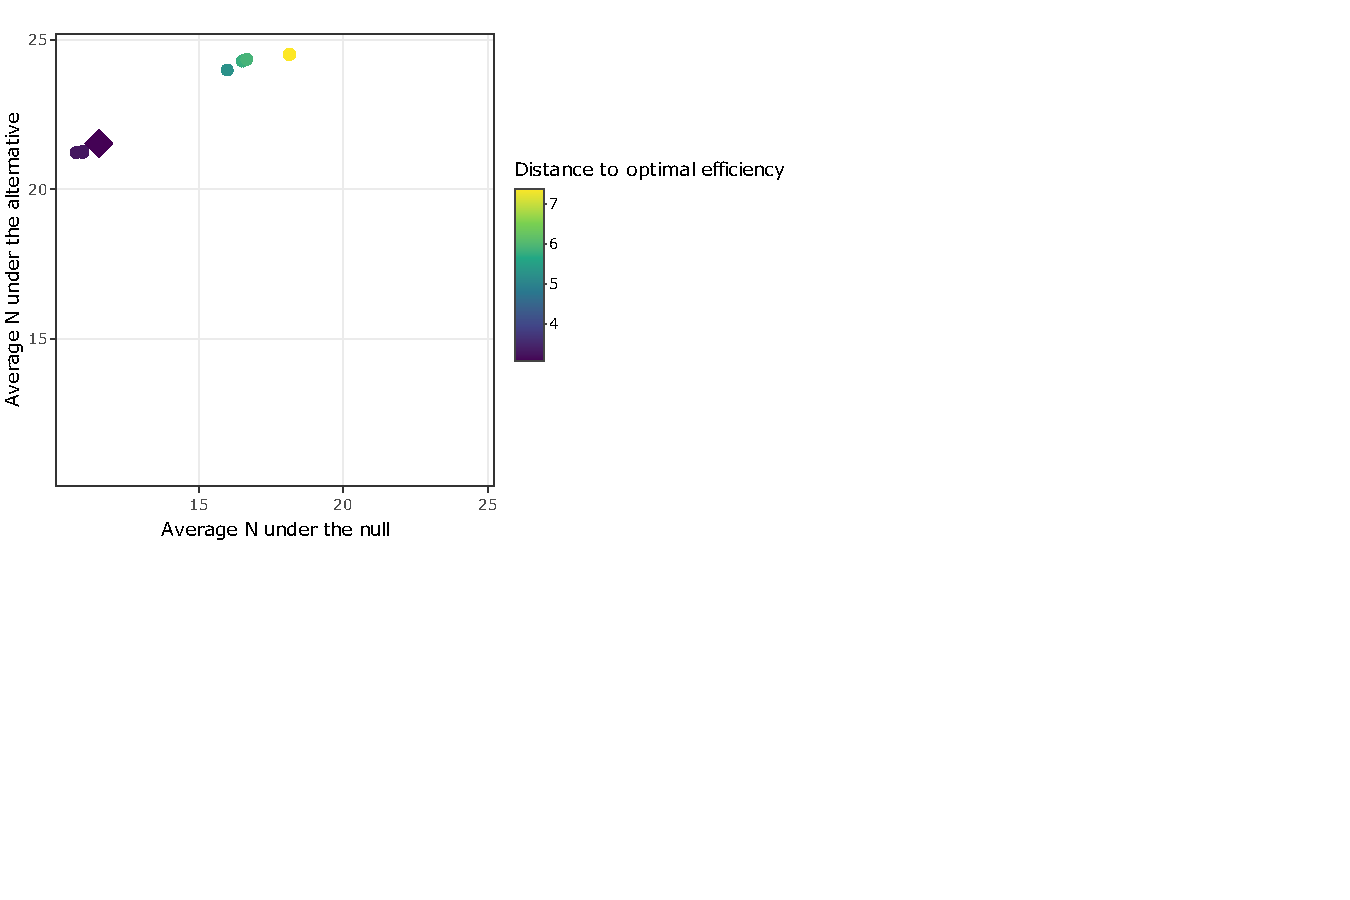
\includegraphics{zabor-hobbs-kane_files/figure-latex/unnamed-chunk-7-2} \end{Schunk}

In this case we may choose to use the optimal efficiency design, which
has the desirable trait of a very small average sample size under the
null of just 39 patients, while still maintaining reasonable type I
error of 0.06 and power of 0.796. This design would allow us to stop
early if the treatment were inefficacious, thus preserving valuable
financial resources for use in studying more promising treatments and
preventing our human subjects from continuing an ineffective treatment.
Finally, we generate the decision table associated with the selected
design for use in making decision at each interim analysis during the
conduct of the trial. Because of the computational time involved, the
results of the below example code are available as a dataset called
\code{one\_sample\_decision\_tbl} included in the \pkg{ppseq} package.
In the results table, we see that at the first interim futility look
after just 5 patients, we would not stop the trial. After the first 10
patients we would stop the trial if there were 0 responses, and so on.
At the end of the trial when all 95 patients have accrued, we would
declare the treatment promising of further study if there were
\textgreater=14 responses.

\begin{Schunk}
\begin{Sinput}
set.seed(123)

one_sample_decision_tbl <- 
  calc_decision_rules(
    n = seq(5, 95, 5),
    N = 95, 
    theta = 0.92, 
    ppp = 0.1, 
    p0 = 0.1, 
    direction = "greater",
    delta = NULL, 
    prior = c(0.5, 0.5), 
    S = 5000
    )
\end{Sinput}
\end{Schunk}

\begin{Schunk}
\begin{Sinput}
one_sample_decision_tbl
\end{Sinput}
\begin{Soutput}
#> # A tibble: 19 x 3
#>        n     r     ppp
#>    <dbl> <int>   <dbl>
#>  1     5    NA NA     
#>  2    10     0  0.0634
#>  3    15     0  0.022 
#>  4    20     1  0.0844
#>  5    25     1  0.0326
#>  6    30     2  0.0702
#>  7    35     2  0.0288
#>  8    40     3  0.0536
#>  9    45     4  0.0708
#> 10    50     4  0.0344
#> 11    55     5  0.0478
#> 12    60     6  0.0622
#> 13    65     7  0.0888
#> 14    70     8  0.095 
#> 15    75     8  0.033 
#> 16    80     9  0.0326
#> 17    85    10  0.0346
#> 18    90    11  0.0162
#> 19    95    13  0
\end{Soutput}
\end{Schunk}

\begin{Schunk}
\begin{Sinput}
plot(one_sample_decision_tbl)
\end{Sinput}

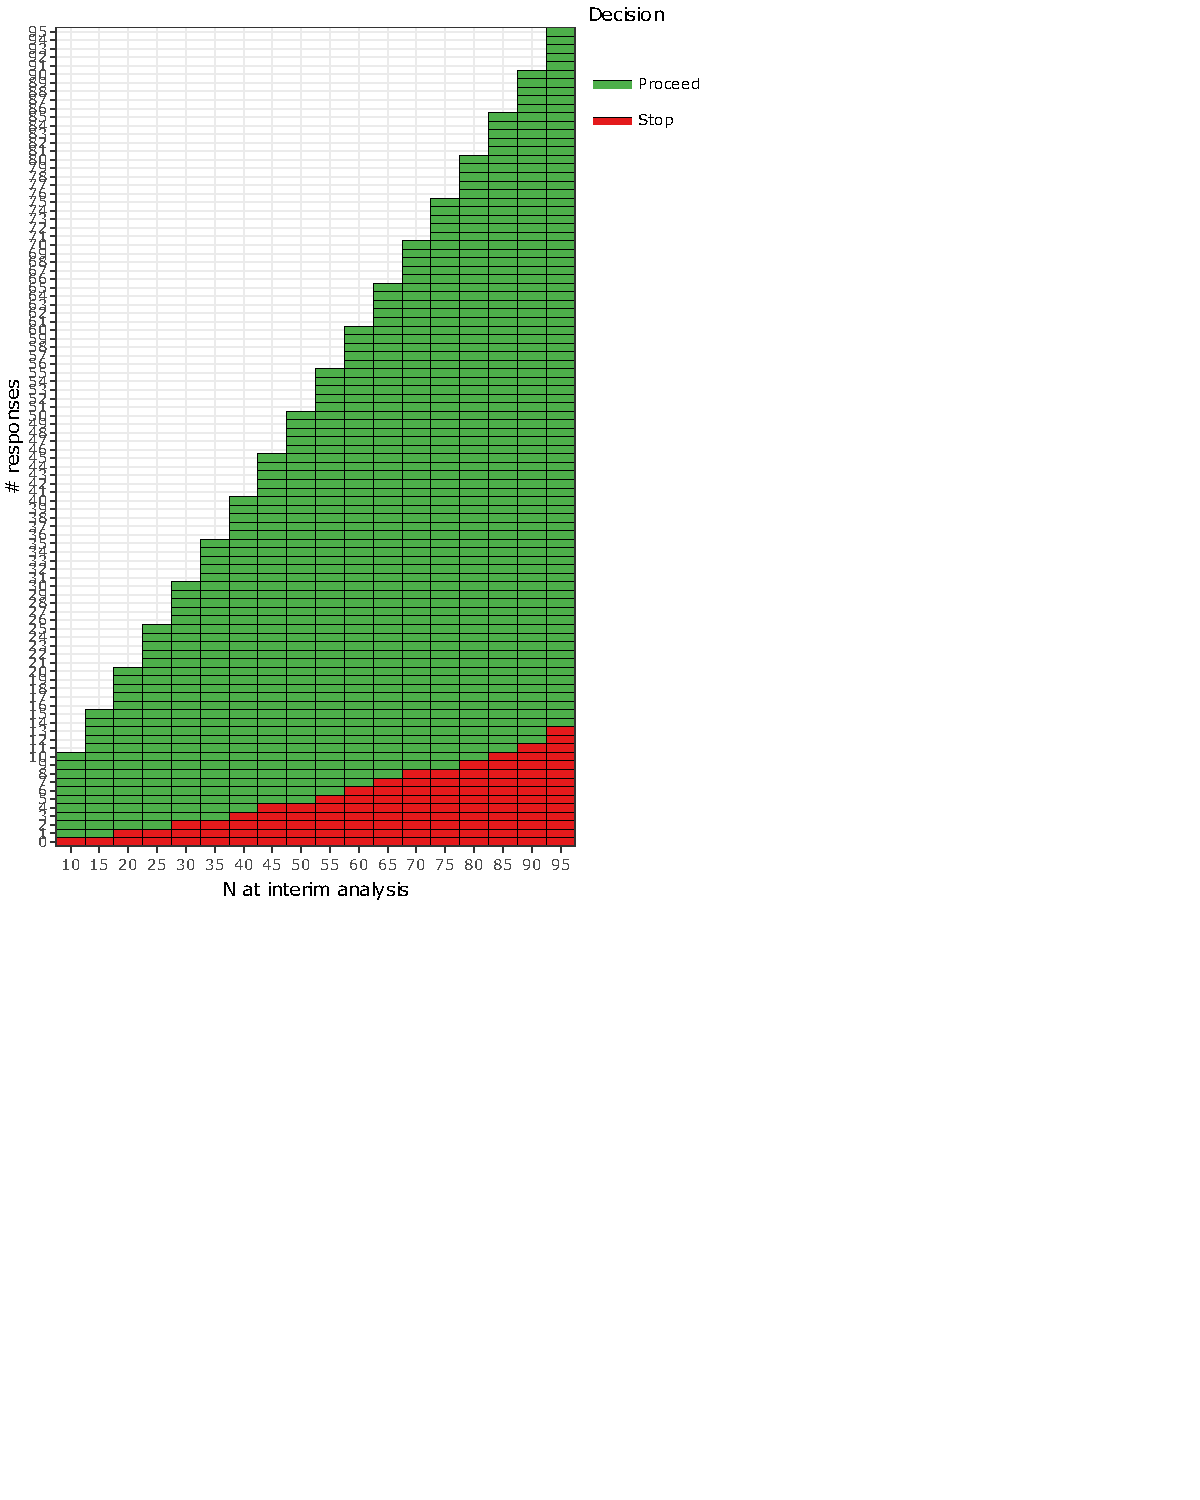
\includegraphics{zabor-hobbs-kane_files/figure-latex/unnamed-chunk-10-1} \end{Schunk}

\hypertarget{summary}{%
\section{Summary}\label{summary}}

With the focus of early stage clinical trial research in oncology
shifting away from the study of cytotoxic treatments and toward
immunotherapies and other non-cytotoxic treatments, new approaches to
clinical trial design are needed that move beyond the traditional search
for the maximum tolerated dose. Bayesian sequential predictive
probability monitoring provides a natural and flexible way to expand the
number of patients studied in phase 1 or to design phase 2 trials that
allow for efficient early stopping for futility while maintaining
control of type I error and power. The \pkg{ppseq} package implements
functionality to consider a range of posterior and predictive thresholds
for a given study design and identify the optimal design based on
accuracy (i.e.~type I error and power) or efficiency (i.e.~average
sample sizes under the null and alternative). Interactive visualization
options are provided to ease comparison of the resulting design options.
Once an ideal design is selected, a table of decision rules can be
obtained to make trial conduct simple and straightforward.

\bibliography{zabor-hobbs-kane.bib}

\address{%
Emily C. Zabor\\
Department of Quantitative Health Sciences \& Taussig Cancer Institute,
Cleveland Clinic\\%
9500 Euclid Ave. CA-60\\ Cleveland, OH 44195 USA\\
%
\url{http://www.emilyzabor.com/}\\%
\textit{ORCiD: \href{https://orcid.org/0000-0002-1402-4498}{0000-0002-1402-4498}}\\%
\href{mailto:zabore2@ccf.org}{\nolinkurl{zabore2@ccf.org}}%
}

\address{%
Brian P. Hobbs\\
Dell Medical School, The University of Texas at Austin\\%
true\\ Austin, TX 78712\\
%
%
\textit{ORCiD: \href{https://orcid.org/0000-0003-2189-5846}{0000-0003-2189-5846}}\\%
\href{mailto:brian.hobbs@austin.utexas.edu}{\nolinkurl{brian.hobbs@austin.utexas.edu}}%
}

\address{%
Michael J. Kane\\
Department of Biostatistics, Yale University\\%
22 Mill Pond Drive\\ Guilford, CT 06437\\
%
%
\textit{ORCiD: \href{https://orcid.org/0000-0003-1899-6662}{0000-0003-1899-6662}}\\%
\href{mailto:michael.kane@yale.edu}{\nolinkurl{michael.kane@yale.edu}}%
}
